\section{Выполнение работы в microcap}

\begin{figure}[H]
	\centering
	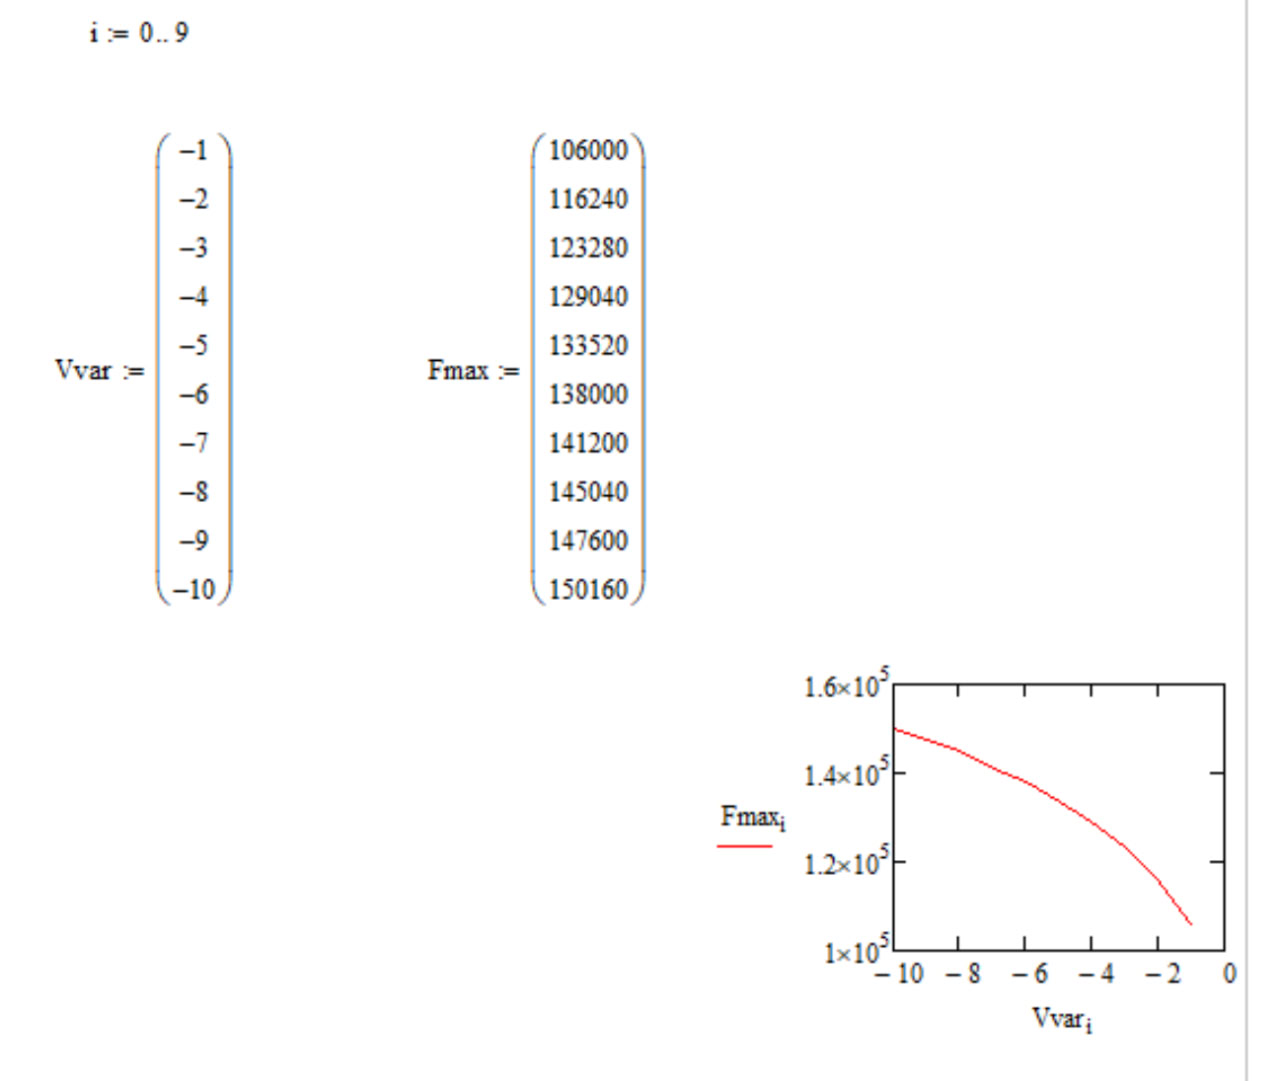
\includegraphics[width=0.77\textwidth]{img/08.jpg}
	\captionsetup{font=footnotesize}
	\caption{Перенос данных в mathcad}
	\label{fig:08}
\end{figure}

\begin{figure}[H]
	\centering
	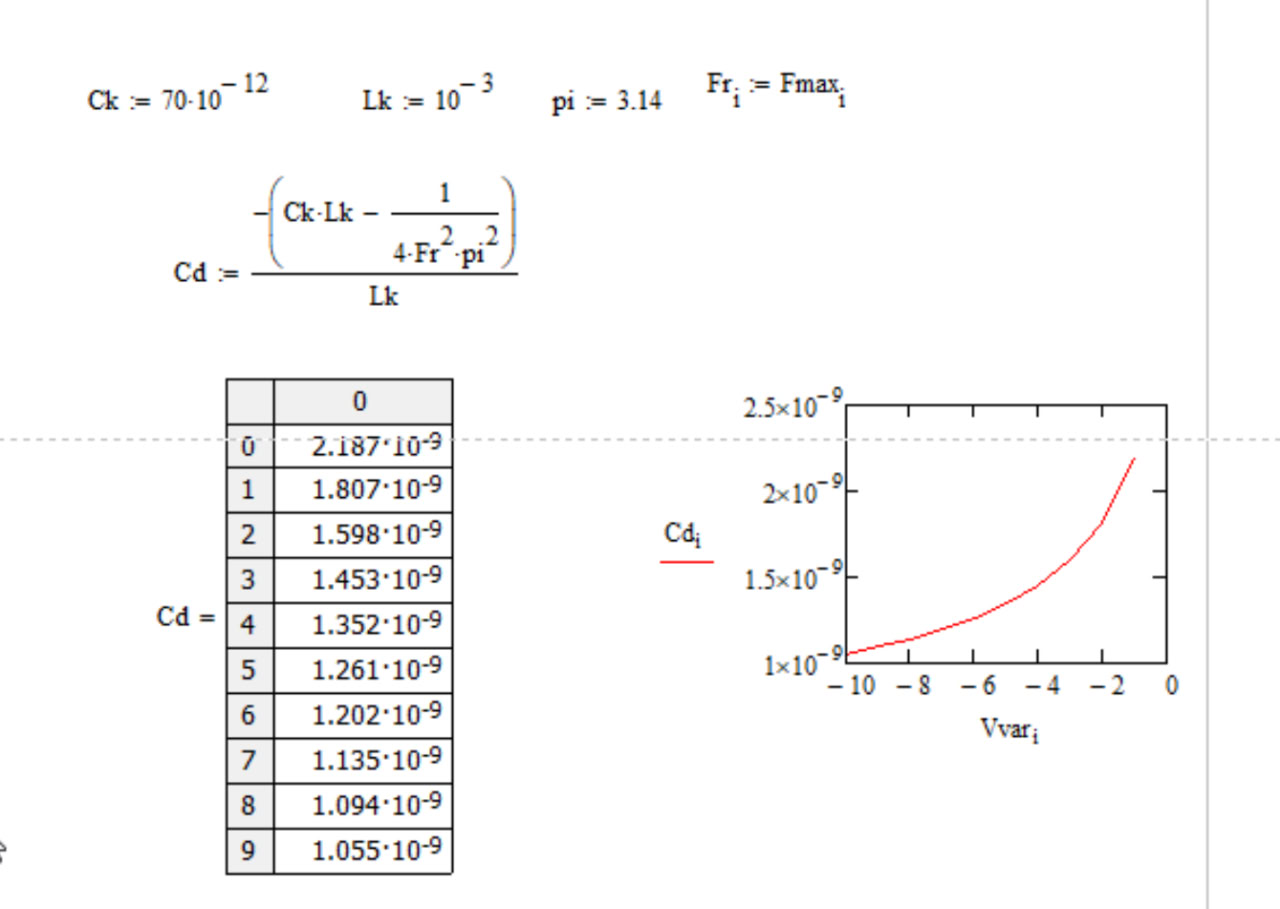
\includegraphics[width=0.77\textwidth]{img/09.jpg}
	\captionsetup{font=footnotesize}
	\caption{Расчёт барьерной ёмкости}
	\label{fig:09}
\end{figure}

Для вычисления параметров барьерной ёмкости по указанной формуле можно использовать метод решения системы нелинейных уравнений, применяя вычислительный блок \textbf{Given-Minerr}.

\begin{figure}[H]
	\centering
	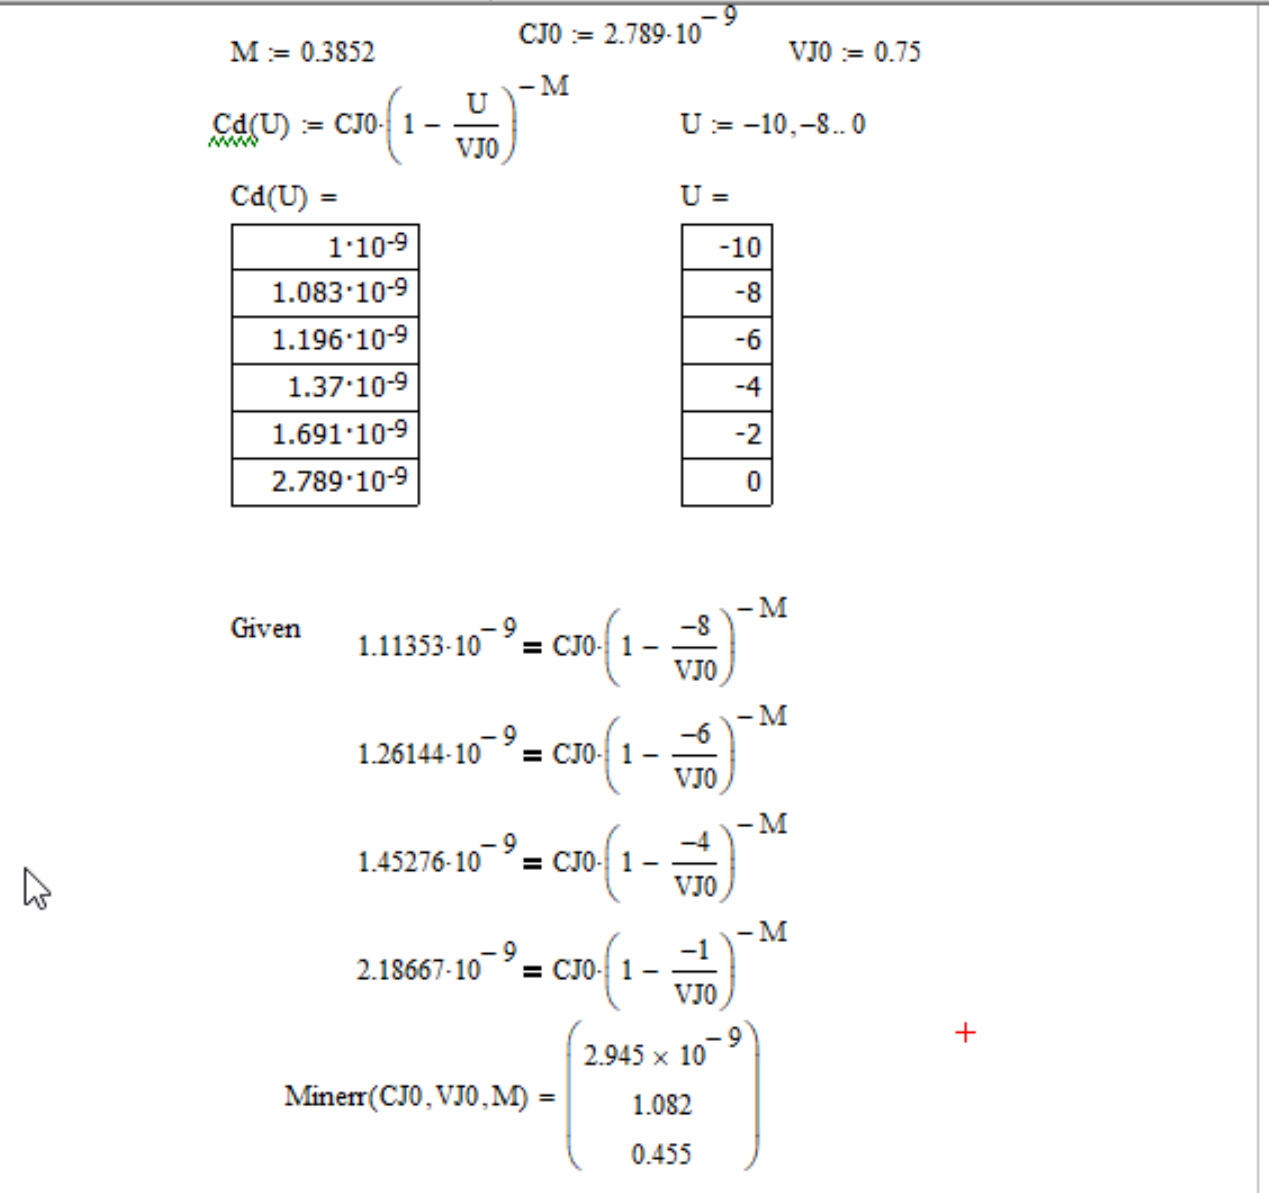
\includegraphics[width=0.9\textwidth]{img/10.jpg}
	\captionsetup{font=footnotesize}
	\caption{Результат вычислений методом Given-Minerr}
	\label{fig:10}
\end{figure}

\subsection{Сравнение результатов}

\begin{tabular}{|c|c|c|}
	\hline
	Характеристики & Исходные данные &  Вычисленные данные \\
	\hline
	CJ0 & 2.789n & 2,945n \\
	\hline
	VJ0 &0.75& 1.082 \\
	\hline
	M & 0.3852& 0.455 \\
	\hline
\end{tabular}
\newline
\newline
Как видно, полученные данных слегка отличаются от исходных.

\begin{figure}[H]
	\centering
	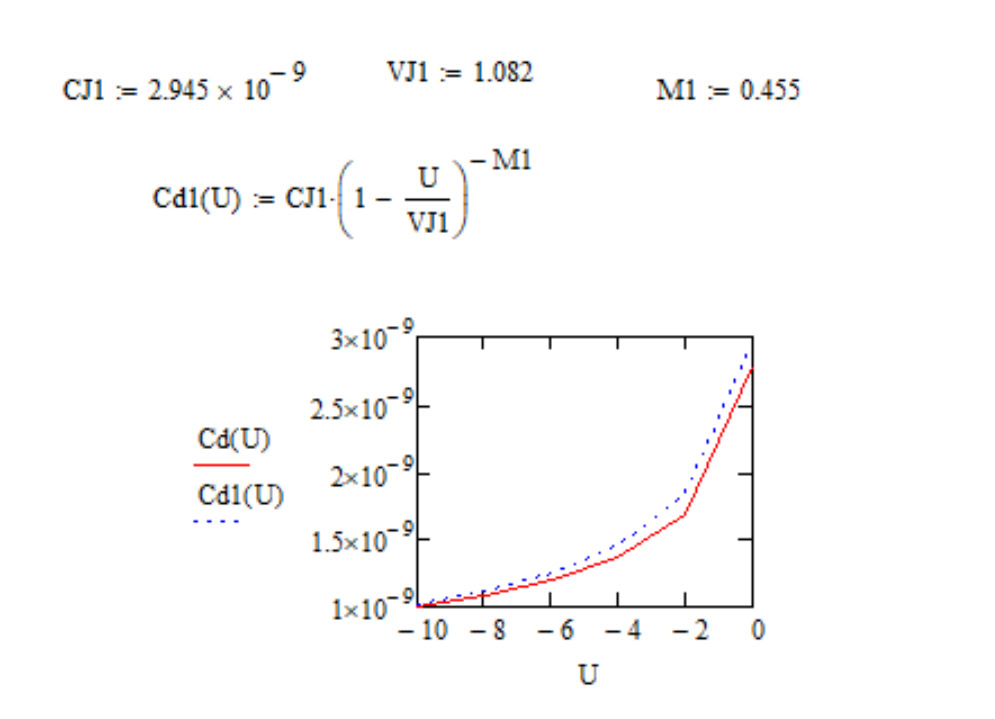
\includegraphics[width=1\textwidth]{img/11.jpg}
	\captionsetup{font=footnotesize}
	\caption{Наложение графиков}
	\label{fig:11}
\end{figure}